\chapter[Simulado4]{Simulado}
\markboth{Simulado 4}{}

\num{1} Leia os textos a seguir e responda à pergunta:

\begin{quote}
\textbf{TEXTO 1}\\
\textbf{Nova imagem da Via Láctea mostra mais de 3 bilhões de
estrelas}

Endereço do Sistema Solar, a Via Láctea contém centenas de bilhões de
estrelas, regiões cintilantes de formação estelar e enormes nuvens
escuras de poeira e gás. Catalogar esses objetos é uma tarefa trabalhosa
e longa, mas o segundo conjunto de dados da Pesquisa com Câmera de
Energia Escura (DECaPS2) revelou recentemente um número impressionante
desses corpos celestes em detalhes nunca antes vistos. {[}...{]}.

Apesar dos desafios, os astrônomos foram capazes de espiar através de
grande parte da poeira que absorve a luz usando equipamentos de
infravermelho. Os pesquisadores também usaram uma abordagem inovadora de
processamento de dados, que lhes permitiu prever melhor o fundo por trás
de cada estrela.

{[}...{]}

\fonte{Veja. Nova imagem da Via Láctea mostra mais de 3 bilhões de estrelas. Disponível em: \emph{https://veja.abril.com.br/ciencia/nova-imagem-da-via-lactea-mostra-mais-de-3-bilhoes-de-estrelas/}.
Acesso em: 26 fev. 2023.}
\end{quote}

\begin{quote}
\textbf{TEXTO 2}\\
\textbf{Levantamento inédito da Via Láctea revela 3,3 bilhões
de objetos celestes}

Astrônomos divulgaram um novo levantamento sobre os objetos celestes
que compõem a Via Láctea. Obtidos por meio do Plano Galáctico com a
Câmera de Energia Escura (DECaPS2), os dados inéditos apresentam
impressionantes 3,32 bilhões de formações que incluem estrelas, regiões
cintilantes de formação estelar e enormes nuvens escuras de poeira e
gás.

{[}...{]}

“Uma das principais razões para o sucesso do DECaPS2 é que simplesmente
apontamos para uma região com uma densidade extraordinariamente alta de
estrelas {[}...{]}”, disse Andrew Saydjari, aluno de pós-graduação da
Universidade Harvard e principal autor do artigo.

{[}...{]}.

\fonte{Galileu. Levantamento inédito da Via Láctea revela 3,3 bilhões de objetos celestes.
Disponível em: \emph{https://revistagalileu.globo.com/ciencia/espaco/noticia/2023/01/levantamento-inedito-da-via-lactea-revela-33-bilhoes-de-objetos-celestes.ghtml}.
Acesso: 26 fev. 2023.}
\end{quote}

\pagebreak
No tratamento das informações, uma vantagem do texto 2 em relação ao texto é que ele

\begin{escolha}
\item foi publicado em site mais conhecido.

\item trata de um assunto sério.

\item apresenta a fala de um especialista.

\item é mais longo e complexo.
\end{escolha}

\coment{SAEB: Avaliar a fidedignidade de informações sobre um mesmo fato
veiculadas em diferentes mídias. BNCC: EF05LP16 – Comparar informações
sobre um mesmo fato veiculadas em diferentes mídias e concluir sobre
qual é mais confiável e por quê.}

\num{2} Leia o texto.

\begin{quote}
{[}...{]} A mão era bonita, tão bonita como o dono; mas parece que
\textbf{ele} estava menos preocupado com a ferida da mão que com o
amarrotado dos punhos {[}...{]}.

\fonte{Machado de Assis. \emph{Várias histórias.} Disponível em:
\emph{https://machado.mec.gov.br/obra-completa-lista/item/download/26\_29eaa69154e158508ef8374fcb50937a}.
Acesso em: 26 fev. 2023.}
\end{quote}

O pronome destacado se refere a qual termo antecedente?

\begin{minipage}{.5\textwidth}
\begin{escolha}
\item Mão

\item Dono

\item Mas

\item Era
\end{escolha}
\end{minipage}
\sidetext{SAEB: Identificar os mecanismos de referenciação lexical e pronominal.
BNCC: EF05LP27 – Utilizar, ao produzir o texto, recursos de coesão
pronominal (pronomes anafóricos) e articuladores de relações de sentido
(tempo, causa, oposição, conclusão, comparação), com nível adequado de
informatividade.}

\pagebreak
\num{3} Leia o texto a seguir e responda à pergunta:

\begin{quote}
\textbf{Moradores registram a última superlua do ano no centro-oeste
paulista}

Moradores de várias cidades do interior de São Paulo registraram a
superlua {[}...{]}.

A superlua ocorre quando o satélite natural surge “maior” no céu.
Segundo os astrônomos, isso ocorre porque a lua está em seu ponto da
órbita mais próximo da Terra, chamado de perigeu.

{[}...{]}

Esta superlua de agosto é conhecida como “Superlua de Esturjão”. O
nome está relacionado à época em que o peixe é encontrado em bastante
quantidade nos Grandes Lagos da América do Norte, um conjunto imenso de
lagos de água doce entre o Canadá e os Estados Unidos.
{[}...{]}.
\end{quote}

\fonte{G1. Moradores registram a última superlua do ano no centro-oeste paulista; veja as fotos. Disponível em: \emph{https://g1.globo.com/sp/bauru-marilia/noticia/2022/08/12/moradores-registram-a-ultima-superlua-do-ano-no-centro-oeste-paulista-veja-as-fotos.ghtml}.
Acesso em: 26 fev. 2023.}

De acordo com o texto, a superlua ocorre porque

\begin{escolha}
\item a lua está em seu ponto da órbita mais próximo da Terra.

\item o fenômeno pode ser observado em vários países.

\item muitas pessoas registram o fenômeno.

\item o fato coincide com ao aumento da população de esturjão.
\end{escolha}

\coment{SAEB: Analisar relações de causa e consequência. BNCC: EF05LP27 -
Utilizar, ao produzir o texto, recursos de coesão pronominal (pronomes
anafóricos) e articuladores de relações de sentido (tempo, causa,
oposição, conclusão, comparação), com nível adequado de informatividade.}

\pagebreak
\num{4} Leia o trecho.

\begin{quote}
Os cabelos, apanhados no alto da cabeça por um pedaço de fita
enxovalhada, faziam-lhe um solidéu natural, cuja borla era suprida por
um \textbf{raminho} de arruda.

\fonte{Joaquim Maria Machado de Assis. \emph{Esaú e Jacó.}
Disponível em:
\emph{https://machado.mec.gov.br/obra-completa-lista/item/download/12\_ab2c739d2e8293712078e7b6b0c12abb}.
Acesso em: 26 fev. 2023.}
\end{quote}

Na palavra destacada, a terminação \textbf{-inho} indica algo

\begin{minipage}{.5\textwidth}
\begin{escolha}
\item pequeno.

\item grande.

\item positivo.

\item irrelevante.
\end{escolha}
\end{minipage}
\sidetext{SAEB: Reconhecer em textos o significado de palavras derivadas a partir
de seus afixos. BNCC: EF05LP08 – Diferenciar palavras primitivas,
derivadas e compostas, e derivadas por adição de prefixo e de sufixo.}

\num{5} Leia o trecho.

\begin{quote}
{[}...{]} – Vem comigo, disse eu, arranjei recursos... temos muito
dinheiro, terás tudo o que quiseres... Olha, toma {[}...{]}.

\fonte{Joaquim Maria Machado de Assis. \emph{Memórias póstumas de
Brás Cubas.} Disponível em:
\emph{https://machado.mec.gov.br/obra-completa-lista/item/download/16\_ff646a924421ea897f27cf6d21e6bb23}.
Acesso em: 26 fev. 2023.}
\end{quote}

A partir do trecho, podemos inferir que o termo “recursos” tem sentido próximo ao de

\begin{minipage}{.5\textwidth}
\begin{escolha}
\item “vir”.

\item “comigo”.

\item “arranjar”.

\item “dinheiro”.
\end{escolha}
\end{minipage}
\sidetext{SAEB: Inferir o sentido de palavras ou expressões em textos. BNCC:
EF35LP05 – Inferir o sentido de palavras ou expressões desconhecidas em
textos, com base no contexto da frase ou do texto.}

\pagebreak
\num{6} Leia o texto.

\begin{quote}
\textbf{Startup quer treinar abelhas para polinizarem café com maior precisão}\\

{[}...{]}

Assim como os cães, as abelhas podem ser treinadas para desempenhar
tarefas de farejamento, como reconhecer com precisão a fragrância de
culturas agrícolas de interesse econômico, como o café (\textit{Coffea arabica}),
e, dessa forma, polinizá-las com maior eficácia. Isso porque esses
insetos polinizadores têm capacidade de desenvolver memória olfativa
{[}...{]}.

Com base nessas constatações, corroboradas durante seu doutorado em
ecologia na Universidade Estadual de Campinas (Unicamp) e em
neurociências na Université Paul Sabatier, em Toulouse, na França,
[o pesquisador] fundou em parceria com Marcela Barbosa, doutora em entomologia
pela Universidade de São Paulo de Ribeirão Preto (USP), e Maria
Imaculada Zucchi, professora da Unicamp e pesquisadora da Agência
Paulista de Tecnologia do Agronegócio (APTA), Polo Piracicaba, uma
\textit{startup}, batizada de PollinTech, voltada a melhorar a precisão da
polinização do café por abelhas africanizadas.

{[}...{]}.

\fonte{Elton Alisson. Veja. Startup quer treinar abelhas para polinizarem café com maior precisão. Disponível em:
\emph{https://veja.abril.com.br/ciencia/startup-quer-treinar-abelhas-para-polinizarem-cafe-com-maior-precisao/}.
Acesso em: 26 fev. 2023.}
\end{quote}

De modo geral, o texto trata

\begin{escolha}
\item dos estudos sobre abelhas no Brasil.

\item do crescimento de \textit{startups} no Brasil.

\item da agressividade das abelhas que se encontram no Brasil.

\item da iniciativa de treinar abelhas para melhorar a polinização do café.
\end{escolha}

\coment{SAEB: Identificar a ideia central o texto. BNCC: EF35LP03 – Identificar
a ideia central do texto, demonstrando compreensão global.}

\pagebreak
\num{7} Leia o texto.

\begin{quote}
\textbf{Nasa diz que 2022 foi o quinto ano mais quente da história}

{[}...{]}

Ao examinar dados de temperatura da superfície terrestre ao longo do ano
[de 2022], cientistas do Goddard Institute for Space Studies (GISS), da
Nasa, descobriram que 2022 empatou com 2015 como o quinto mais quente já
registrado.

{[}...{]}

“Essa tendência de aquecimento é alarmante”, disse o chefe da agência
espacial americana, Bill Nelson. “Nosso aquecimento climático já está
deixando uma marca: os incêndios florestais estão se intensificando; os
furacões estão ficando mais fortes; as secas estão causando estragos, e
o nível do mar está subindo”.

{[}...{]}

\fonte{Veja. Nasa diz que 2022 foi o quinto ano mais quente da história. Disponível em:
\emph{https://veja.abril.com.br/ciencia/nasa-diz-que-2022-foi-o-quinto-ano-mais-quente-da-historia/}.
Acesso em: 26 fev. 2023.}
\end{quote}

De acordo com o texto, uma das consequências do aquecimento global é

\begin{escolha}
\item a criação de um instituto de estudos espaciais.

\item a pesquisa sobre os anos mais quentes da história.

\item o aumento do número de incêndios florestais.

\item a diminuição da ocorrência de furacões.
\end{escolha}

\coment{SAEB: Localizar informação explícita. BNCC: EF15LP03 – Localizar informações explícitas em textos.}

\pagebreak
\num{8}  Observe a fotografia.

\begin{figure}[htpb!]
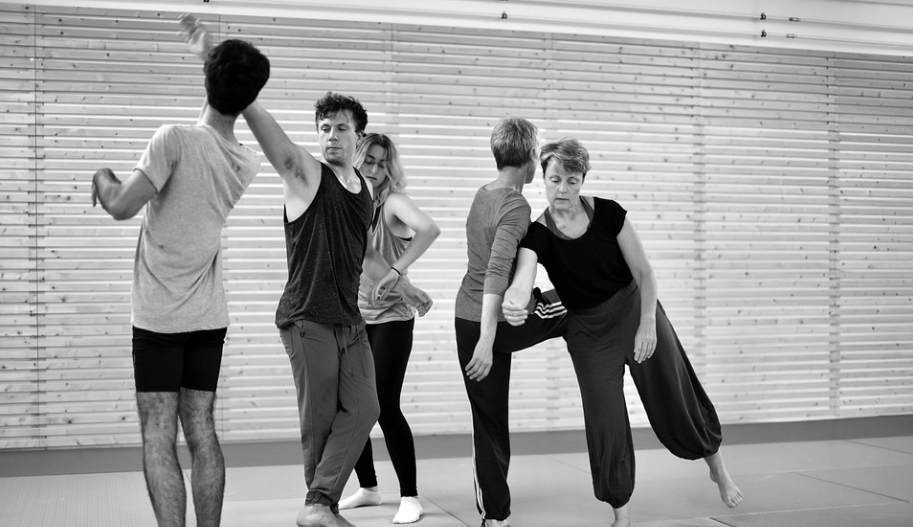
\includegraphics[width=\textwidth]{./imgs/art39.png}
\caption{Improvisação de contato na dança.}
\end{figure}
%\emph{https://cdn.pixabay.com/photo/2018/09/17/19/59/contact-improvisation-3684693_960_720.jpg}

A improvisação é uma característica da dança contemporânea, que também tem como característica o fato de

\begin{minipage}{.5\textwidth}
\begin{escolha}
\item
  possuir técnica e vocabulário próprios.
\item
  não possuir limitação de movimentos.
\item
  contar com roupas e acessórios padronizados.
\item
  empregar postura ereta e verticalizada.
\end{escolha}
\end{minipage}
\sidetext{SAEB: Identificar distintas formas e/ou gêneros de expressão da dança,
da música e do teatro em diferentes contextos e práticas.
BNCC: EF15AR08 – Experimentar e apreciar formas distintas de
manifestações da dança presentes em diferentes contextos, cultivando a
percepção, o imaginário, a capacidade de simbolizar e o repertório
corporal.}

\num{9}  Leia a descrição de um instrumento musical.

De matriz africana, chegou ao Brasil pelas mãos dos escravizados saídos de Angola
e é um dos mais importantes instrumentos musicais brasileiros. É o principal
elemento musical de uma roda de capoeira, controlando seu ritmo.

A descrição corresponde à de

\begin{minipage}{.5\textwidth}
\begin{escolha}
\item
  um pandeiro.
\item
  um berimbau.
\item
  um cavaquinho.
\item
  uma cuíca.
\end{escolha}
\end{minipage}
\sidetext{SAEB: Identificar as características de instrumentos musicais
variados, bem como o potencial musical do corpo humano.}

\pagebreak
\num{10} Assinale a alternativa que contém um exemplo de patrimônio imaterial brasileiro.

\begin{escolha}
\item
  Centro Histórico de Ouro Preto, em Minas Gerais.
\item
  Ruínas de São Miguel das Missões, no Rio Grande do Sul.
\item
  Praça São Francisco em São Cristóvão, em Sergipe.
\item
  Festa do Divino Espírito Santo de Pirenópolis, de Goiás.
\end{escolha}

\coment{SAEB: Avaliar nas linguagens artísticas a diversidade do patrimônio
cultural da humanidade (material e imaterial), em especial o brasileiro,
a partir de suas diferentes matrizes.
BNCC: EF15AR25 – Conhecer e valorizar o patrimônio cultural, material e
imaterial, de culturas diversas, em especial a brasileira, incluindo-se
suas matrizes indígenas, africanas e europeias, de diferentes épocas,
favorecendo a construção de vocabulário e repertório relativos às
diferentes linguagens artísticas.}

%\chapter{Simulado 4}
%\begin{figure}[htpb!]
%\vspace*{-3cm}
%\hspace*{-2.5cm}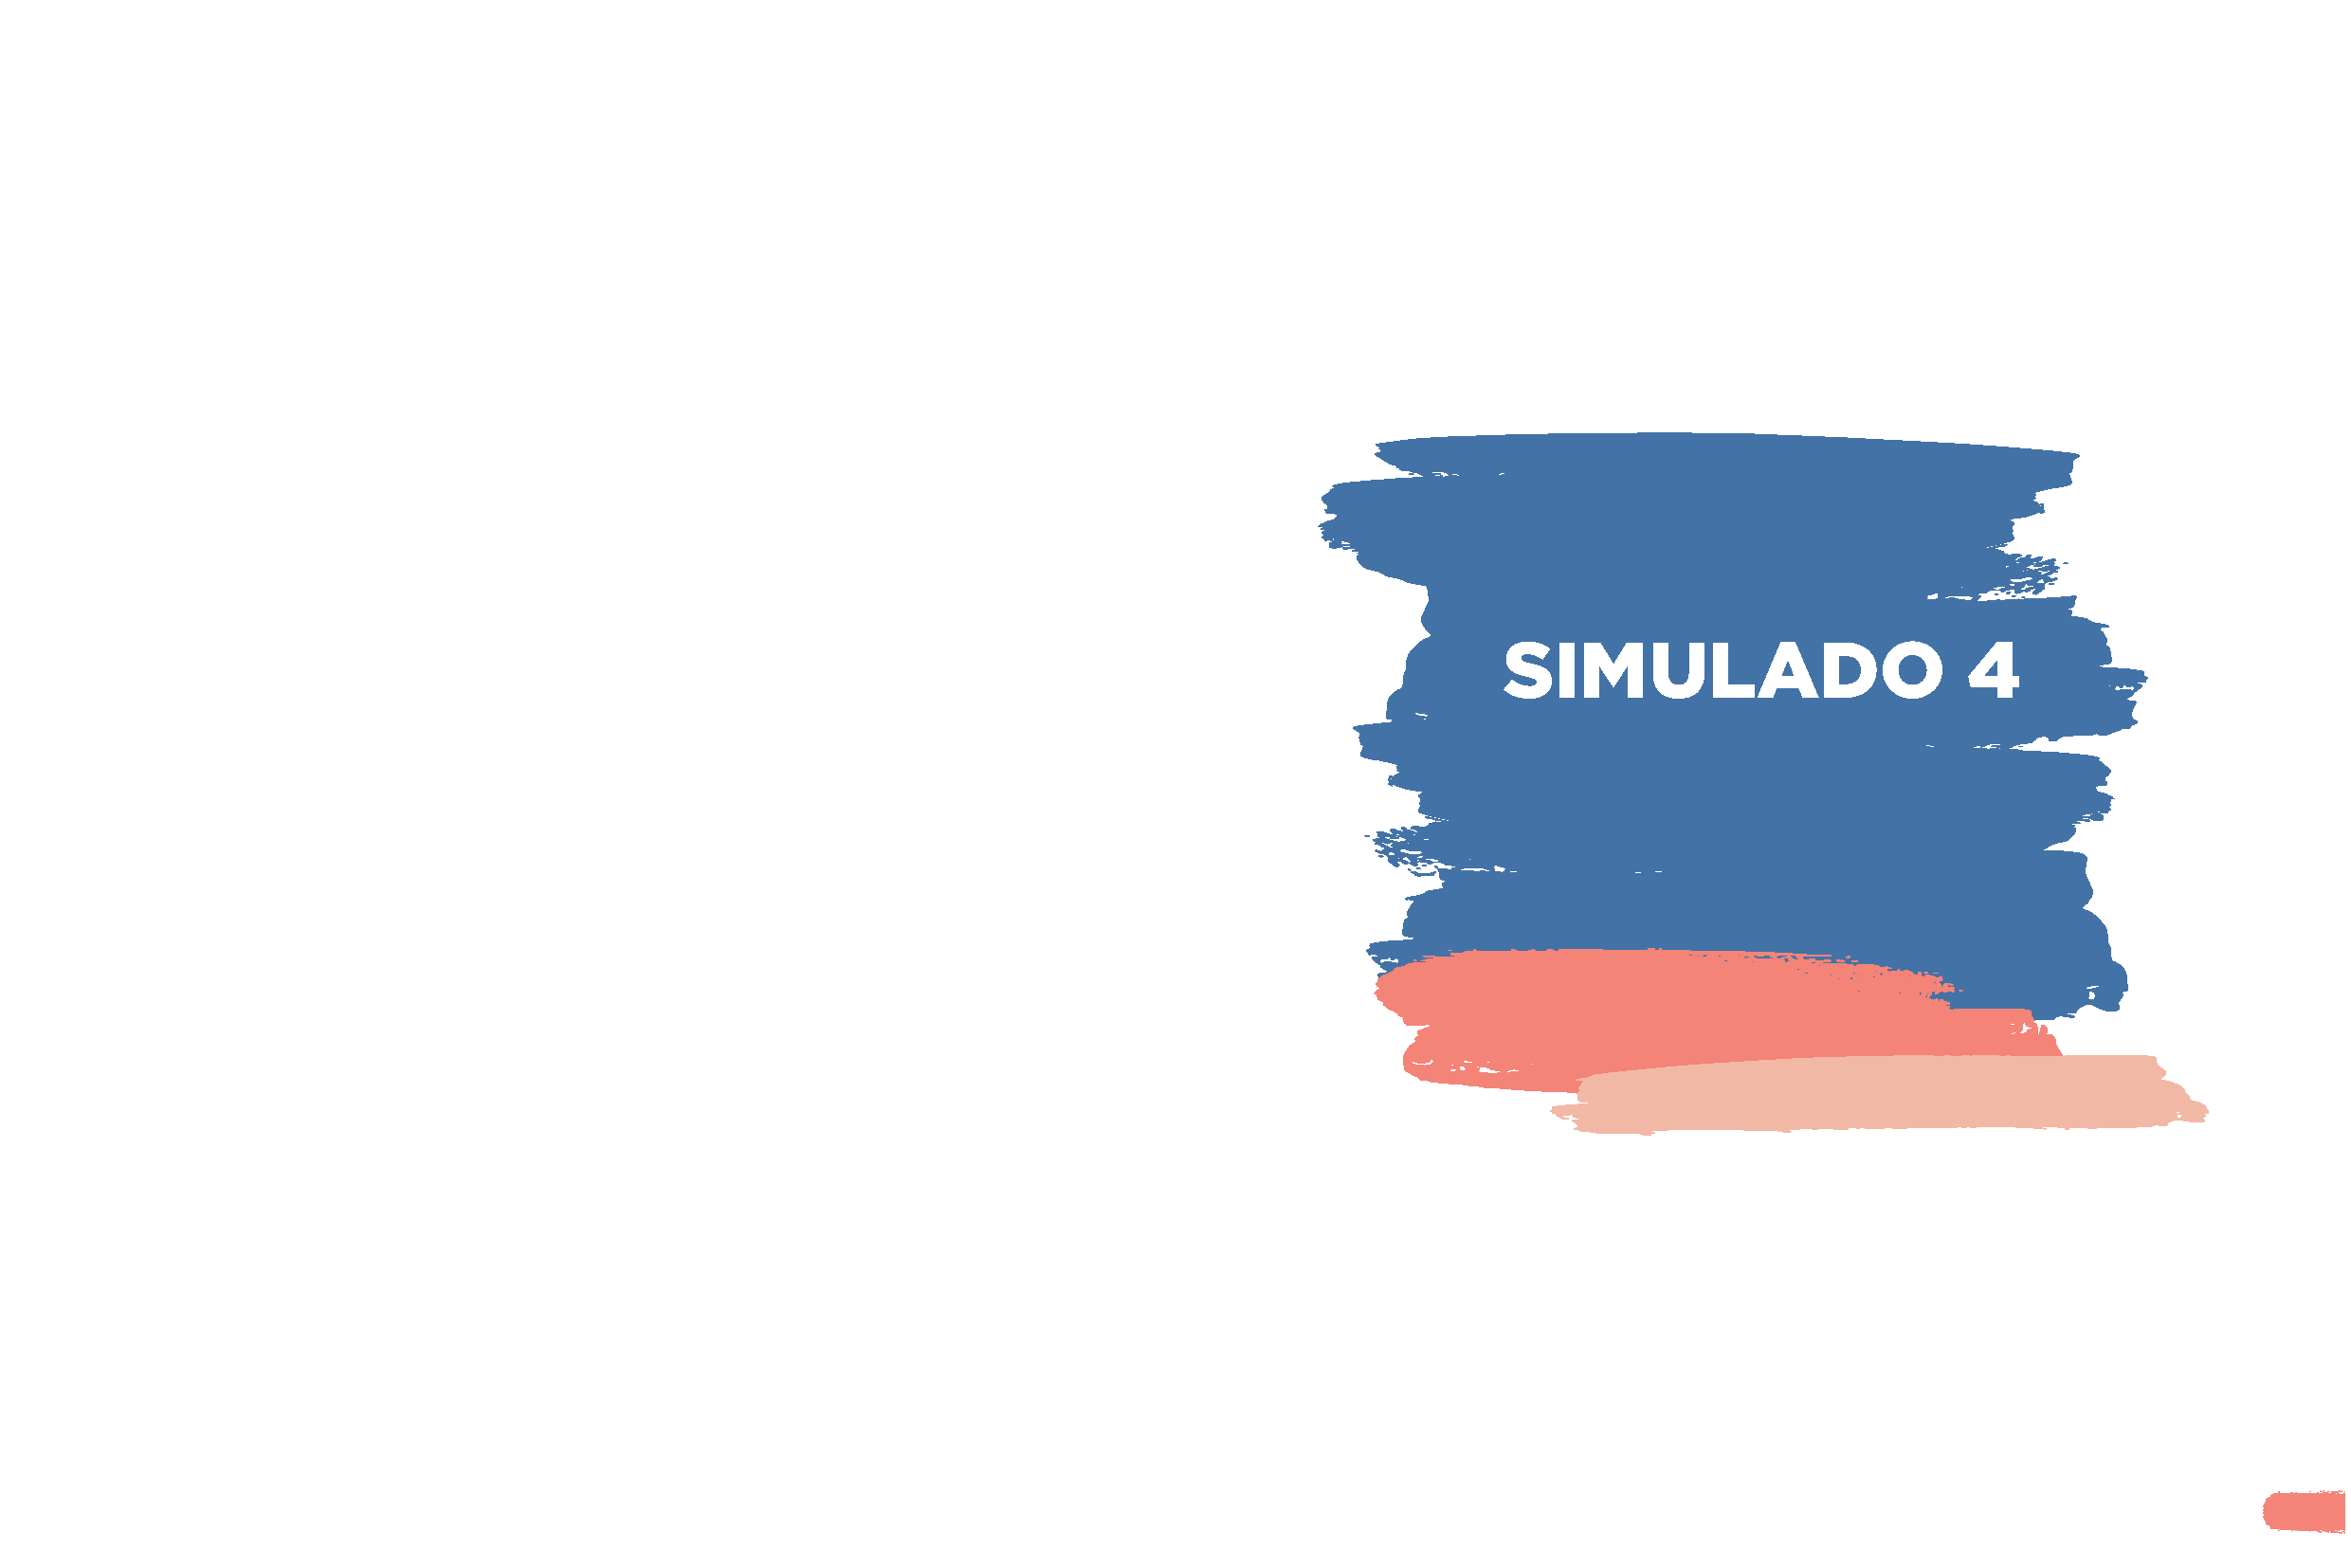
\includegraphics[scale=1]{../watermarks/4simulado5ano.pdf}
%\end{figure}
%
%\newwatermark[pagex={69,71}]{\vspace{2.5cm}\hspace*{8cm}\includegraphics[scale=1]{../watermarks/%bgsim5anoimpar.pdf}}
%\newwatermark[pagex={70}]{\vspace{2.5cm}\hspace*{7.8cm}\includegraphics[scale=1]{../watermarks/%bgsim5anopar.pdf}}
%
%\pagebreak
%\movetooddpage
%\markboth{Simulado 2}{}

\num{11}

\begin{figure}[htpb!]

\includegraphics[width=.5\textwidth]{./imgs/img69.png}
\end{figure}
%Disponível em: \emph{https://br.freepik.com/vetores-gratis/mao-com-calendario-de-marca-de-caneta\_1250622.htm\#query=calend\%C3\%A1rio\&position=18\&from\_view=search\&track=sph} Acesso em: 23 fev. 2023.

A imagem apresentada anteriormente representa o seguinte marcador temporal:

\begin{minipage}{.5\textwidth}
\begin{escolha}
\item o relógio.

\item a ampulheta.

\item o diário.

\item o calendário
\end{escolha}
\end{minipage}
\sidetext{BNCC: EF05HI07 - Identificar os processos de produção, hierarquização e
difusão dos marcos de memória e discutir a presença e/ou a ausência de
diferentes grupos que compõem a sociedade na nomeação desses marcos de
memória.}

\pagebreak
\num{12}

\begin{quote}
\textbf{Expansão urbana global ameaça 205 espécies de animais, diz estudo}

Até 2030, novas cidades do planeta ocuparão 1,2 milhão de km² de área.
Mata Atlântica, Cerrado e outros biomas do mundo podem ser degradados.
Um novo estudo realizado por pesquisadores norte-americanos afirma que
até 2030, 1,2 milhão de km² do planeta deixarão de ser áreas preservadas
para dar lugar a grandes cidades – uma área equivalente ao dobro do
tamanho do estado da Bahia. {[}\ldots{}{]}
A partir da análise, os especialistas
afirmam que é preciso desenvolver projetos sustentáveis para os próximos
28 anos, o que evitaria um grande impacto ao meio ambiente e às futuras
gerações humanas. {[}\ldots{}{]}

\fonte{Do Globo Natureza, em São Paulo. G1. Expansão urbana global ameaça 205 espécies de animais, diz estudo. Disponível em:
\emph{https://g1.globo.com/natureza/noticia/2012/09/expansao-urbana-global-ameaca-205-especies-de-animais-diz-estudo.html}.
Acesso em: 24 mar. 2023.}
\end{quote}

\noindent{}Segundo o texto, a expansão urbana global ameaça os animais, pois o
aumento das cidades

\begin{escolha}
\item diminui a área de plantações de alimento.

\item melhora a condição de vida dos humanos.

\item invade os territórios onde eles habitam.

\item baixa a destruição das florestas.
\end{escolha}

\coment{BNCC: EF05GE03 - Identificar as formas e funções das cidades e
analisar as mudanças sociais, econômicas e ambientais provocadas pelo
seu crescimento.}

\num{13}

\begin{quote}
Talvez você já tenha parado para refletir sobre o porquê de as religiões de matriz africana serem o principal alvo de intolerância religiosa no Brasil.
É um fato que uma das vertentes desse problema são os rastros deixados pela escravidão, da época em que o Brasil era ainda uma colônia, em que pessoas eram rotuladas como inferiores simplesmente por terem origem africana e nada mais.
E o problema não parece estar perto de ter uma solução. Dados do Disque 100 (da Secretaria Nacional de Direitos Humanos) apontam 697 casos de intolerância religiosa entre 2011 e 2015.
\end{quote}

\fonte{Fonte de pesquisa: Jefferson Puff. Da BBC Brasil, Rio de Janeiro. Por que as religiões de matriz africana são o principal alvo de intolerância no Brasil?. Disponível em:
\emph{https://bbc.in/2JX0KVz}.
Acesso em: 24 mar. 2023.}

Segundo o texto, um dos motivos da discriminação contra as religiões
citadas no texto é

\begin{escolha}
\item a falta de denúncias contra crimes de intolerância.

\item a diversidade cultural ensinada nas escolas públicas.

\item a violência de grupos descendentes de ex-escravos.

\item o preconceito com a comunidade afro-brasileira.
\end{escolha}

\coment{BNCC: EF05GE02 - Identificar diferenças étnico-raciais e étnico-culturais
e desigualdades sociais entre grupos em diferentes territórios.}

\num{14}

\begin{quote}
No Brasil, é o IPHAN (Instituto do Patrimônio Histórico e Artístico Nacional) o órgão que cuida da preservação do Patrimônio Cultural. Cabe
a ele promover as riquezas culturais do nosso país, garantindo que elas estejam disponíveis tanto para as gerações atuais quanto para as futuras gerações de brasileiros.
\end{quote}

\noindent{}Um exemplo de local que pode ser protegido pelo IPHAN é

\begin{minipage}{.5\textwidth}
\begin{escolha}
\item um condomínio de casas.

\item uma plantação de arroz.

\item uma igreja muito antiga.

\item uma floresta no litoral.
\end{escolha}
\end{minipage}
\sidetext{BNCC: EF05HI02 - Identificar os mecanismos de organização do poder
político com vistas à compreensão da ideia de Estado e/ou de outras
formas de ordenação social.}

\pagebreak
\num{15}

\begin{quote}
\textbf{Copa do Mundo: entenda as denúncias sobre direitos humanos contra o Catar }

Desde que foi escolhido como sede da Copa, em 2010, país sofre críticas
sobre tratamento das mulheres, membros da comunidade LGBT, trabalhadores
migrantes e jornalistas, por exemplo. {[}\ldots{}{]}
As mulheres no Catar {[}\ldots{}{]}
enfrentam discriminação generalizada tanto na lei quanto na prática. {[}\ldots{}{]}
Pelas denúncias que envolvem os direitos humanos, a seleção da Dinamarca
pretendia usar camisetas durantes seus treinos na Copa do Mundo com
mensagem em prol dos direitos humanos. {[}\ldots{}{]}

\fonte{CNN. Copa do Mundo: entenda as denúncias sobre direitos humanos contra o Catar. Disponível em:
\emph{https://www.cnnbrasil.com.br/esporte/copa-do-mundo-entenda-as-denuncias-sobre-direitos-humanos-contra-o-catar/}.
Acesso em: 23 fev. 2023.}
\end{quote}

Segundo a notícia, o direito humano que não estaria sendo seguido
pelo governo do Catar é o direito

\begin{minipage}{.5\textwidth}
\begin{escolha}
\item de proteção contra a tortura.

\item à moradia.

\item à nacionalidade.

\item à igualdade.
\end{escolha}
\end{minipage}
\sidetext{BNCC: EF05HI04 - Associar a noção de cidadania com os princípios de
respeito à diversidade, à pluralidade e aos direitos humanos.}
